\documentclass[10pt]{article}

\usepackage[utf8]{inputenc}
\usepackage{latexsym,amsfonts,amssymb,amsthm,amsmath}
\setlength{\parindent}{0in}
\setlength{\parskip}{\baselineskip}
\setlength{\oddsidemargin}{0in}
\setlength{\textwidth}{6.5in}
\setlength{\textheight}{8.8in}
\setlength{\topmargin}{0in}
\setlength{\headheight}{18pt}

\usepackage[a4paper,margin=1in,footskip=0.25in]{geometry}

\usepackage{listings}
\usepackage{color} %red, green, blue, yellow, cyan, magenta, black, white
\definecolor{mygreen}{RGB}{28,172,0} % color values Red, Green, Blue
\definecolor{mylilas}{RGB}{170,55,241}

\usepackage{graphicx}
\graphicspath{{../writeup/}}

\title{PHYS 410 Homework 1}
\author{Gavin Pringle, 56401938}

%%%%%%%%%%%%%%%%%%%%%%%%%%%%%%%%%%%%%%%%%%%%%%%%%%%%%%%%%%%%%%%%%%%%%%%%%%%%%%%%%%%%%%%%%%%%%%%%%%%%%%%
% Start of document
%%%%%%%%%%%%%%%%%%%%%%%%%%%%%%%%%%%%%%%%%%%%%%%%%%%%%%%%%%%%%%%%%%%%%%%%%%%%%%%%%%%%%%%%%%%%%%%%%%%%%%%
\begin{document}

\maketitle

\lstset{language=Matlab,%
    %basicstyle=\color{red},
    breaklines=true,%
    morekeywords={matlab2tikz},
    keywordstyle=\color{blue},%
    morekeywords=[2]{1}, keywordstyle=[2]{\color{black}},
    identifierstyle=\color{black},%
    stringstyle=\color{mylilas},
    commentstyle=\color{mygreen},%
    showstringspaces=false,%without this there will be a symbol in the places where there is a space
    numbers=left,%
    numberstyle={\tiny \color{black}},% size of the numbers
    numbersep=9pt, % this defines how far the numbers are from the text
    emph=[1]{for,end,break},emphstyle=[1]\color{red}, %some words to emphasise
    %emph=[2]{word1,word2}, emphstyle=[2]{style},    
}

%%%%%%%%%%%%%%%%%%%%%%%%%%%%%%%%%%%%%%%%%%%%%%%%%%%%%%%%%%%%%%%%%%%%%%%%%%%%%%%%%%%%%%%%%%%%%%%%%%%%%%%
% Introduction
%%%%%%%%%%%%%%%%%%%%%%%%%%%%%%%%%%%%%%%%%%%%%%%%%%%%%%%%%%%%%%%%%%%%%%%%%%%%%%%%%%%%%%%%%%%%%%%%%%%%%%%
\subsection*{Introduction}
In this homework assignment, two methods for solving nonlinear equations numerically via root finding 
are explored: bisection and Newton's method. In order to do this, two problems are provided. The first 
problem involves the 1-dimesional case where the roots of a nonlinear function are found using a hybrid 
algorithm that first employs bisection followed by Newton's method. The second problem involves the 
d-dimensional case where a nonlinear system is solved using a d-dimensional Newton iteration. 

In both problems it is assumed the function and its derivative in problem 1 as well as the system of 
equations and its Jacobian in problem 2 are hard-coded as Matlab functions. Specifically, a polynomial
of order 10 is provided for the first question and a nonlinear system of three variables is provided 
for the second question. 

\pagebreak

%%%%%%%%%%%%%%%%%%%%%%%%%%%%%%%%%%%%%%%%%%%%%%%%%%%%%%%%%%%%%%%%%%%%%%%%%%%%%%%%%%%%%%%%%%%%%%%%%%%%%%%
% Problem 1 - Hybrid Algorithm
%%%%%%%%%%%%%%%%%%%%%%%%%%%%%%%%%%%%%%%%%%%%%%%%%%%%%%%%%%%%%%%%%%%%%%%%%%%%%%%%%%%%%%%%%%%%%%%%%%%%%%%
\subsection*{Problem 1 - Hybrid Algorithm}

\subsubsection*{Review of Theory}

Bisection, also referred to as binary search, is a method used for solving nonlinear equations of the 
form $f(x)=0$ for the 1-dimensional case or $\vec{f}(\vec{x})=\vec{0}$ for the d-dimensional case. The
bisection algorithm involves bisecting a search interval and checking whether the root is above or 
below the bisector. The search interval is then bisected again in the new interval where the root lies, 
and again it is determined whether the root is above or below the new bisector. This process then repeats
until the root is determined to be in an interval of small enough tolerance. 

For the 1-dimensional bisection algorithm, it is assumed that there is a root of $f(x)=0$ in the interval
$x_{min} \leq x \leq x_{max}$. From this, it follows that $f(x_{min})f(x_{max}) \leq 0$. As previously 
described, the interval $[x_{min}, x_{max}]$ which has width $\delta x_0 = x_{max} - x_{min}$ is
successively divided into smaller intervals of width $\delta x_1 = \delta x_0/2$, 
$\delta x_2 = \delta x_0/4$, $\delta x_3 = \delta x_0/8$, \ldots each of contains the root which is 
checked using the condition $f({x_{min}}^{(n)})f({x_{max}}^{(n)}) \leq 0$. This process is continued until 
interval is suitably small, which is verified by checking the relative error given by the formula
$\frac{| \delta x^{(n)} |}{| x^{(n+1)} |} \leq \epsilon$

Newton's method is another 

\subsubsection*{Numerical Approach}

definition of all pertinent problem parameters

exposition of the requisite equations

methodology that is used to solve the problem

function signature 

testing method 

provided equations

\subsubsection*{Implementation}

refer to appendix 

iteration counter

\subsubsection*{Results}

graph and console output 

\begin{figure}[h!]
\centering
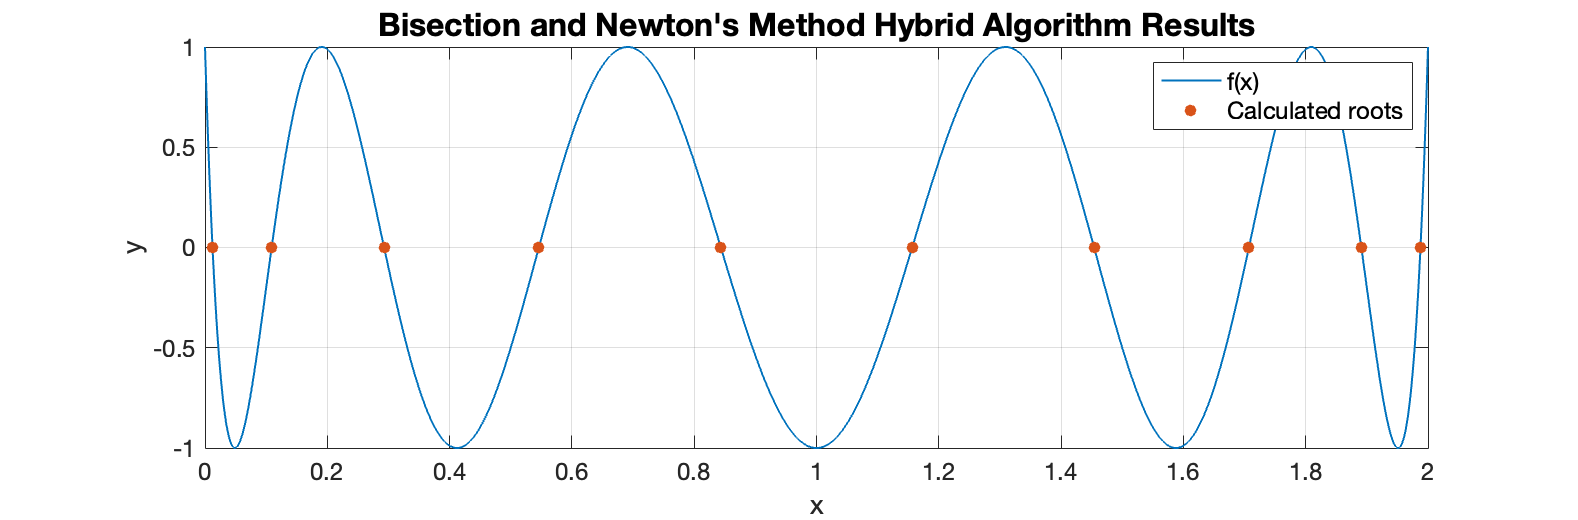
\includegraphics[width=1\textwidth]{HybridPlot.png}
\caption{Numerically calculated roots overlaid on example function $f(x)$.}
\end{figure}

\pagebreak

%%%%%%%%%%%%%%%%%%%%%%%%%%%%%%%%%%%%%%%%%%%%%%%%%%%%%%%%%%%%%%%%%%%%%%%%%%%%%%%%%%%%%%%%%%%%%%%%%%%%%%%
% Problem 2 - D-dimesional Newton's Method
%%%%%%%%%%%%%%%%%%%%%%%%%%%%%%%%%%%%%%%%%%%%%%%%%%%%%%%%%%%%%%%%%%%%%%%%%%%%%%%%%%%%%%%%%%%%%%%%%%%%%%%
\subsection*{Problem 2 - D-dimesional Newton's Method}

\subsubsection*{Review of Theory}
Go over theory for d-d newton's method: 

\subsubsection*{Numerical approach}

definition of all pertinent problem parameters

exposition of the requisite equations

methodology that is used to solve the problem

function signature 

testing method 

provided equations

\begin{figure}[h!]
\centering
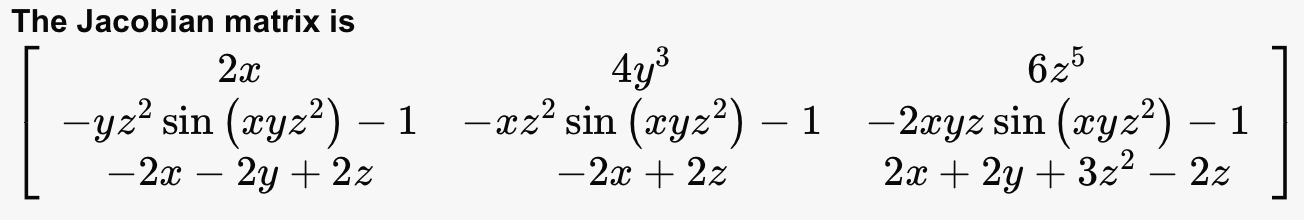
\includegraphics[width=0.75\textwidth]{Jacobian.png}
\caption{Calculated Jacobian matrix for the provided system of equations.}
\end{figure}

\subsubsection*{Implementation}

refer to appendix 

iteration counter

\subsubsection*{Results}

console output

\pagebreak

%%%%%%%%%%%%%%%%%%%%%%%%%%%%%%%%%%%%%%%%%%%%%%%%%%%%%%%%%%%%%%%%%%%%%%%%%%%%%%%%%%%%%%%%%%%%%%%%%%%%%%%
% Conclusions
%%%%%%%%%%%%%%%%%%%%%%%%%%%%%%%%%%%%%%%%%%%%%%%%%%%%%%%%%%%%%%%%%%%%%%%%%%%%%%%%%%%%%%%%%%%%%%%%%%%%%%%
\subsection*{Conclusions}
Briefly summarize your findings (again, more extensively in the case of projects).
Discuss any particular problems you had with the homework/project.
Include your statement concerning your use or non-use of generative AI here.

\pagebreak

%%%%%%%%%%%%%%%%%%%%%%%%%%%%%%%%%%%%%%%%%%%%%%%%%%%%%%%%%%%%%%%%%%%%%%%%%%%%%%%%%%%%%%%%%%%%%%%%%%%%%%%
% Appendix A - Hybrid Algorithm Code
%%%%%%%%%%%%%%%%%%%%%%%%%%%%%%%%%%%%%%%%%%%%%%%%%%%%%%%%%%%%%%%%%%%%%%%%%%%%%%%%%%%%%%%%%%%%%%%%%%%%%%%
\subsection*{Appendix A - Hybrid Algorithm Code}
\lstinputlisting{../hybrid.m}

\pagebreak

%%%%%%%%%%%%%%%%%%%%%%%%%%%%%%%%%%%%%%%%%%%%%%%%%%%%%%%%%%%%%%%%%%%%%%%%%%%%%%%%%%%%%%%%%%%%%%%%%%%%%%%
% Appendix B - D-dimesional Newton's Method Code
%%%%%%%%%%%%%%%%%%%%%%%%%%%%%%%%%%%%%%%%%%%%%%%%%%%%%%%%%%%%%%%%%%%%%%%%%%%%%%%%%%%%%%%%%%%%%%%%%%%%%%%
\subsection*{Appendix B - D-dimesional Newton's Method Code}
\lstinputlisting{../newtond.m}

\pagebreak

%%%%%%%%%%%%%%%%%%%%%%%%%%%%%%%%%%%%%%%%%%%%%%%%%%%%%%%%%%%%%%%%%%%%%%%%%%%%%%%%%%%%%%%%%%%%%%%%%%%%%%%
% Appendix C - Testing Code
%%%%%%%%%%%%%%%%%%%%%%%%%%%%%%%%%%%%%%%%%%%%%%%%%%%%%%%%%%%%%%%%%%%%%%%%%%%%%%%%%%%%%%%%%%%%%%%%%%%%%%%
\subsection*{Appendix C - Testing Code}
\lstinputlisting{../test.m}


\end{document}